\documentclass[final]{beamer}

% ====================
% Packages
% ====================

\usepackage[T1]{fontenc}
\usepackage{lmodern}
\usepackage[size=a0,orientation=portrait,scale=1.2]{beamerposter}
\usetheme{AISystemsLab}
\usecolortheme{AISystemsLab}
\usepackage{graphicx}
\usepackage{booktabs}
\usepackage{tikz}
\usetikzlibrary{positioning, calc}
\usepackage{pgfplots}
\pgfplotsset{compat=1.17}

% ====================
% Lengths
% ====================

% If you have N columns, choose \sepwidth and \colwidth such that
% (N+1)*\sepwidth + N*\colwidth = \paperwidth
\newlength{\sepwidth}
\newlength{\colwidth}
\setlength{\sepwidth}{0.025\paperwidth}
\setlength{\colwidth}{0.3\paperwidth}

\newcommand{\separatorcolumn}{\begin{column}{\sepwidth}\hspace{0.0125\paperwidth}\raisebox{-\height}[0pt][0pt]{\begin{tikzpicture} \draw[dash pattern=on 2pt off 8 pt, ultra thick](0,86) -- (0,0); \end{tikzpicture}}\end{column}}

\newcommand{\separatorcolumnwithoutline}{\begin{column}{\sepwidth}\end{column}}

\newcommand{\separatorblocks}{\vspace{-25 pt}\begin{block}{}\begin{tikzpicture}\draw[dash pattern=on 2pt off 8pt, ultra thick](0,0) -- (22,0); \end{tikzpicture}\end{block}}

% ====================
% Title
% ====================

\title{Ultra-Wideband (UWB) Positioning System\\Based on ESP32 and DWM3000 Modules}

\author{T. Herter \and S. Krebs}
\institute[AI Systems Lab]{AI Systems Lab}

% ====================
% Footer (optional)
% ====================

\footercontent{
  sourcecode:
  
\includegraphics[scale=0.3]{pics/qr_link_repo.png} \hfill
  \hfill
  \parbox{30em}{ Hochschule Konstanz Technik, Wirtschaft und Gestaltung \\ Departement of Electrical Engineering and Information Technology }
}
% (can be left out to remove footer)

% ====================
% Body
% ====================

\begin{document}
\addtobeamertemplate{headline}{}
{
    \begin{tikzpicture}[remember picture,overlay]
      \node [anchor=north west, inner sep=3cm] at ([xshift=-4cm,yshift=1.0cm]current page.north west)
      {
\includegraphics[height=13.0cm]{pics/HTWG_EI_en_Modul_Zusatz_neg_1C.png}
      }; % also try shield-white.eps
      \node [anchor=north east, inner sep=3cm] at ([xshift=3.0cm,yshift=1.5cm]current page.north east)
     {
\includegraphics[height=7.0cm]{pics/HTWG_EI_Modul_Zeichen_neg_2C.png}
      };
    \end{tikzpicture}
}

\begin{frame}[t]
\begin{columns}[t]
\separatorcolumnwithoutline

\begin{column}{\colwidth}

  \begin{block}{Introduction}
    We present an indoor UWB positioning system
    that capitalizes on advanced hardware and sophisticated algorithms,
    resulting in an exceptional level of accuracy and reliability.
  
    Our UWB system comprises six identical boards,
    all based on the ESP32 microcontroller, a versatile
    and powerful platform known for its capabilities in
    wireless communication and processing. These boards
    are equipped with DWM3000 modules from Quorvo,
    renowned for their high-performance UWB capabilities.

    One of these boards is designated as the ”Tag”, responsible for
    initiating Two-way-Ranging (TWR) measurements with the
    remaining five ”Anchor” boards.
    The innovative aspect of our system lies in its ability to perform accurate
    localization without reliance on external infrastructure
    or centralized processing.

    \begin{figure}[H]
      \centering
      \begin{tikzpicture}[
        node distance=1.5cm,
        device/.style={
          align=center, circle, draw, minimum width=.25cm, minimum height=.5cm
        },
        ghost/.style={
          align=center,minimum width=0cm, minimum height=0cm
        },
        label/.style={
          draw, minimum width=2cm, minimum height=0cm, text width=8cm
        },
        >=latex,
      ]
        % Responders with coords
        \node [device] (device2) at (90:5.5cm) {A1};
        \node [ghost, above=.05cm of device2.north] (dev2) {(x:0,y:2,z:2)};
        \node [device] (device3) at (162:5.5cm) {A2};
        \node [ghost, above=.05cm of device3.north] (dev3) {(x:0,y:2,z:2)};
        \node [device] (device4) at (234:5.5cm) {A3};
        \node [ghost, below=.05cm of device4.south] (dev4) {(x:0,y:2,z:2)};
        \node [device] (device5) at (306:5.5cm) {A4};
        \node [ghost, below=.05cm of device5.south] (dev5) {(x:0,y:2,z:2)};
        \node [device] (device6) at (18:5.5cm) {A5};
        \node [ghost, below=.05cm of device6.south] (dev6) {(x:0,y:2,z:2)};
    
        %Initiator
        \node [device] (device1) at (0,0) {T1};
    
        % TWRs
        \draw [<->] (device1) -- (device2); 
        \draw [<->] (device1) -- (device3); 
        \draw [<->] (device1) -- (device4); 
        \draw [<->] (device1) -- (device5); 
        \draw [<->] (device1) -- node[midway, above, align=left] {TWR} (device6);
    
        %legend
        \node [label] (legend) at (8,5) {AX = Anchor X \\TY = Tag Y};
    
      \end{tikzpicture}
      \caption{Systemarchitecture for Positioning}
    \end{figure}
  \end{block}

  \separatorblocks
  
  \begin{block}{Hardware}
    The hardware design of our system draws inspiration from pre-existing DWM3000 Evaluation
    boards \cite{Makerfabs_2023}.
    However, our proprietary board development enables specialized component selection
    tailored to their intended use cases.
    User-friendliness was a paramount consideration during the design process,
    resulting in the integration of multiple user buttons and LEDs.
    Additionally, the PCB incorporates a convenient LiPo battery charging capability
    via USB-C.

    \begin{figure}
      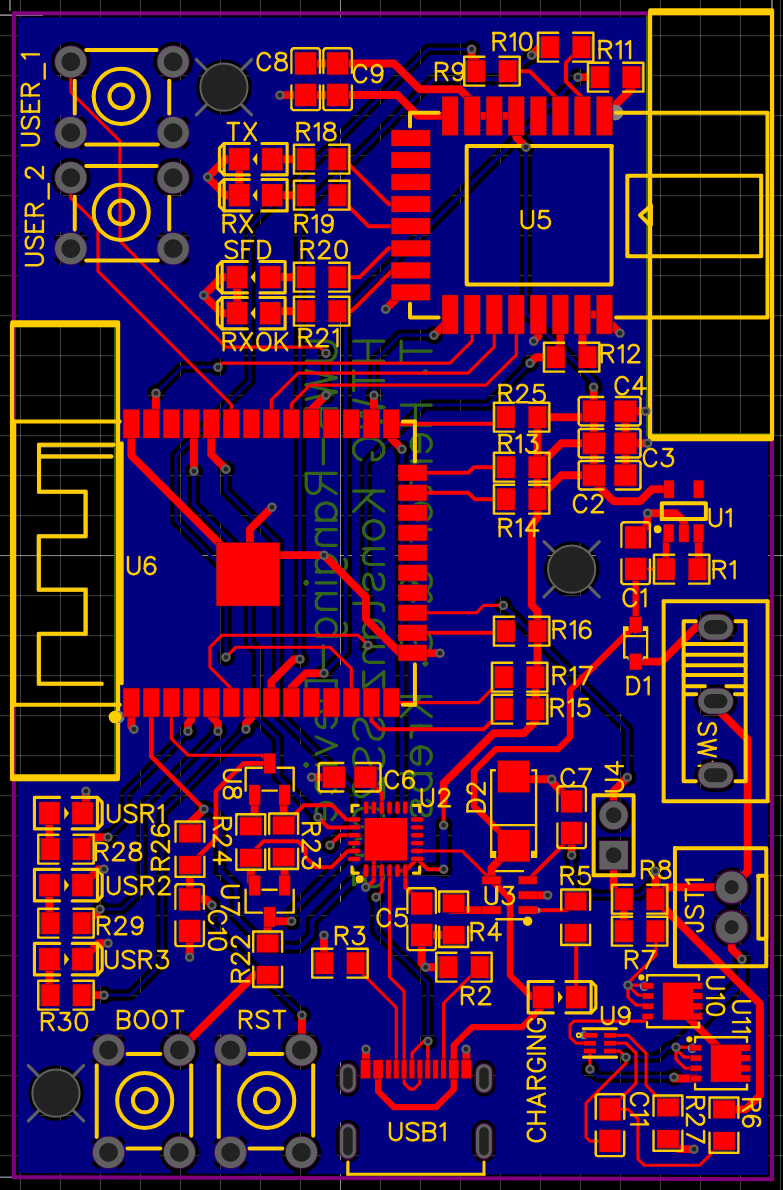
\includegraphics[scale=0.8, angle=90]{pics/pcb_design.png}
      \caption{PCB-Design for UWB Device}
    \end{figure}

    Notably, our PCB design ensures a consistent layout across all boards,
    regardless of their specific application.
    Below the antennas of both the DWM3000 and ESP32,
    the ground plate has been selectively omitted to enhance antenna radiation
    characteristics and enable more precise measurements.
    This meticulous hardware design approach not only optimizes
    performance but also prioritizes user convenience. 
  \end{block}
\end{column}

\separatorcolumn

\begin{column}{\colwidth}

  \begin{block}{Two-way-Ranging (TWR)}
    Two-Way Ranging (TWR) is our foundational technique for obtaining precise
    distance measurements within the UWB positioning system.
    It relies on the time it takes for signals to travel from a Tag board to
    Anchor boards and back again.
    \begin{figure}[H]
      \begin{tikzpicture}[
        node distance=1.5cm,
        block/.style={
          align=center, draw,line width=0.5mm, minimum width=6.85cm, minimum height=.5cm
        },
        ghost/.style={
          align=center,minimum width=0cm, minimum height=0cm
        },
        label/.style={
          minimum width=6cm, minimum height=0cm, text width=6cm
        },
        >=latex,
      ]
        % textfields
        \node [block] (tag_timestamp) {Tag\\Timestamp};
        \node [block, right=2cm of tag_timestamp] (anchor_timestamp) {Anchor\\Timestamp};
    
        % Endpoints
        \node [ghost, below=8cm of tag_timestamp] (tag_endpoint) {};
        \node [ghost, below=8cm of anchor_timestamp] (anchor_endpoint) {};
    
        % Timelines
        \draw [line width=0.5mm, -] (tag_timestamp) -- (tag_endpoint);
        \draw [line width=0.5mm, -] (anchor_timestamp) -- (anchor_endpoint);
    
        % Labels Tag-line
        \node [label, align=right, anchor=east, below=2cm of tag_timestamp.west] (t_send_poll) {$t_{send-poll}$\\$(t_{sp})$};
        \node [label, align=right, anchor=east, below=7cm of tag_timestamp.west] (t_receive_response) {$t_{receive-response}$\\$(t_{rr})$};
        
        % Labels Anchor-line
        \node [label, align=left, anchor=west, below=3cm of anchor_timestamp.east] (t_receive_poll) {$t_{receive-poll}$\\$(t_{rp})$};
        \node [label, align=left, anchor=west, below=6cm of anchor_timestamp.east] (t_send_response) {$t_{send-response}$\\$(t_{sr})$};
    
        %Dotted lines
        \draw [line width=0.5mm, ->] (t_send_poll.east) -- (t_receive_poll.west);
        \draw [line width=0.5mm, ->] (t_send_response.west) -- (t_receive_response.east);
        \node [ghost, below=2.25cm of anchor_timestamp.west] (poll_label) {Poll (ID)};
        \node [ghost, below=6.5cm of tag_timestamp.east] (response_label) {Response};
    
      \end{tikzpicture}
      \caption{Timingdiagram of Two-Way-Ranging}
    \end{figure}

    Given the timestamps the Tag is able to calculate the corresponding
    time-of-flight aswell as the distance between both devices by using the following Formula:

    \begin{equation*}
      \begin{aligned}
        t_{tof} &= \frac{(t_{rp} - t_{sp})+(t_{rr} - t_{sr})}{2}\\
        dist &= t_{tof} * v_{light}\\
        v_{light} &\approxeq 299.792.458,0 \frac{m}{s}
      \end{aligned}
    \end{equation*}

    Using this technique the standarddeviation of die distance estimation
    is approximatly between 4cm to 10cm, depending on the conditions of measurement.
    The estimation error increases significantly if there is a non-line-of-sight condition.

  \end{block}

  \separatorblocks

  \begin{block}{Firmware}
    The Firmware \cite{uwb-tracking} for both the Tags and Anchors shares a common codebase
    with only a minor distinction during device startup.
    Upon booting, the current role of the device is read from the EEPROM,
    and based on this role, the appropriate tasks are executed.

    The development of firmware built on FreeRTOS\cite{FreeRTOS_2023} offers the capability
    to seemingly execute multiple tasks in parallel.
    Leveraging the dual cores of the ESP32 microcontroller allows us to
    genuinely achieve parallelism.

    The versatility of FreeRTOS enables the design of firmware that
    seamlessly adapts to the requirements of both Tags and Anchors.
    This design approach ensures efficient resource utilization and
    effective task management, ultimately contributing to the system's
    overall performance.
  \end{block}

  \begin{alertblock}{Firmware Tasks:}
    \begin{itemize}
      \item \textbf{TOF-Task}: used for executing UWB measurements, eather as Initator or as Responder.
      \vspace*{1cm}
      \item \textbf{EKF-Task}: combines Distance measurements and creates a position estimation.
      \vspace{1cm}
      \item \textbf{BLE-Task}: opens up a Bluetooth server which serves as configuration and feedback interface.
      \vspace{1cm}
    \end{itemize}
  \end{alertblock}
\end{column}

\separatorcolumn

\begin{column}{\colwidth}

  \begin{block}{Extended-Kalman-Filter}
    The Kalman filter primarily consists of three steps.
    First, the state for the next timeiteration is predicted based on the
    current estimated state.
    Next, a measurement is predicted based on the predicted state.
    Finally, the actual measurement is compared to the predicted measurement,
    and the state estimation is corrected based on the estimation error.
    This process leads to the convergence of the estimation towards the ground truth.\cite{Kalman}

    The following blockdiagram shows how the different steps interact to generate a
    state estimation based on the current measurement.
    \begin{figure}[H]
    
      \begin{tikzpicture}[
          node distance=1.5cm,
          block/.style={
              rectangle, draw, align=center,
              minimum width=3cm, minimum height=1.5cm
          },
          >=latex,
      ]
          % System block
          \node [block] (system) {System};
          \node [left=9cm of system] (uk) {$u_k$};
          \node [right=9cm of system] (zk1) {$z_{k+1}$};
          \node [left=.5cm of system] (x_k) at (system.south west) {$x_{k}$};
          \node [right=.5cm of system] (x_k1) at (system.south east) {$x_{k+1}$};
      
          % Kalman filter blocks
          \node [block, below=3cm of system] (messmodel) {Mess-\\modell};
          \node [block, left=2.5cm of messmodel] (systemmodel) {System-\\modell};
          \node [block, right=3.5cm of messmodel] (correction) {Korrektur};
          \node [right=1.5cm of correction] (x_dach_k1) {$\hat{x}_{k+1}$};
          \node [left=1.5cm of systemmodel] (x_dach_k) at (systemmodel.south west) {$\hat{x}_{k}$};
  
          % Arrows
          \draw [line width=0.5mm, ->] (uk) -- (system);
          \draw [line width=0.5mm, ->] (system.east) -- ++(.5,0) |- (zk1);
      
          \coordinate[right=-8.5cm of system.west] (systemcoord_left);
          \draw [line width=0.5mm, ->] (systemcoord_left) |- (systemmodel.west);
          \draw [line width=0.5mm, ->] (systemmodel.east) -- node[above] {$\hat{x}_{k+1|k}$} (messmodel.west);
          \draw [line width=0.5mm, ->] (messmodel.east) -- node[above] {$\hat{z}_{k+1|k}$} (correction.west);
      
          \coordinate[right=1cm of correction.east] (correctioncoord);
          \draw [line width=0.5mm, ->] (correction.east) -- ++(1,0);
          \coordinate[right=2.5cm of system.east] (systemcoord_right);
          \draw [line width=0.5mm, ->] (systemcoord_right)
              |- ($(systemcoord_right)+(3,0)$)
              |- ($(correction.west)+(-.5,3)$)
              |- ($(correction.west)+(-.5,2)$)
              |- ($(correction.west)+(0,.5)$);
  
          \draw [line width=0.5mm, ->] ($(system.east)+(0,-.5)$)
              |- ($(system.east)+(.75,-0.5)$)
              |- ($(system.east)+(.75,-1.5)$)
              |- ($(system.west)+(-.75,-1.5)$)
              |- ($(system.west)+(-.75,-.5)$)
              |- ($(system.west)+(0,-.5)$);
  
          \draw [line width=0.5mm, ->] (messmodel.west)
              |- ($(messmodel.west)+(-1,0)$)
              |- ($(messmodel.west)+(-1,-2)$)
              |- ($(messmodel.east)+(1,-2)$)
              |- ($(correction.west)+(0,-.5)$);
          
          \draw [line width=0.5mm, ->] (correction.east)
              |- ($(correction.east)+(.5,0)$)
              |- ($(correction.east)+(.5,-2.5)$)
              |- ($(systemmodel.west)+(-1.75,-2.5)$)
              |- ($(systemmodel.west)+(0,-.5)$);
        \end{tikzpicture}
        \caption{Blockschaltbild des Kalman Filters}
    \end{figure}
    In this context, $u_k$ represents control commands that input into the system.
    $z_k$ describes the observed measurement at time $k$, and $x$ represents the
    current system state.
    In the case of our application, $x$ contains the three-dimensional coordinates
    of the tag, and the vector $z$ encompasses all distance measurements
    to the landmarks, which are the anchors.
    Every time a variable is marked with a hat,
    that means that this is an estimation of the given variable.
  \end{block}

  \separatorblocks

  \begin{block}{Tests}

    \begin{table}
      \centering
      \begin{tabular}{l r r c}
        \toprule
        \textbf{Ground-Truth} & \textbf{mean} & \textbf{standarddeviation}\\
        $(x,y,z)$ & $mean(x,y,z)$ & $std(x, y, z)$\\
        \midrule
        $(a,b,c)$ & $(a,b,c)$ & $(a,b,c)$\\
        $(a,b,c)$ & $(a,b,c)$ & $(a,b,c)$\\
        $(a,b,c)$ & $(a,b,c)$ & $(a,b,c)$\\
        $(a,b,c)$ & $(a,b,c)$ & $(a,b,c)$\\
        \bottomrule
      \end{tabular}
      \caption{Presentation of Testresults}
    \end{table}

  \end{block}

  \begin{block}{References}

    \nocite{*}
    \footnotesize{\bibliographystyle{plain}\bibliography{poster}}

  \end{block}

\end{column}

\separatorcolumnwithoutline
\end{columns}
\end{frame}

\end{document}
g
Fusce aliquam magna velit
Et rutrum ex euismod vel. Pellentesque ultricies, velit
in fermentum vestibulum, lectus nisi pretium nibh, sit
amet aliquam lectus augue vel velit. Suspendisse
rhoncus massa porttitor augue feugiat molestie. Sed
molestie ut orci nec malesuada. Sed ultricies feugiat
est fringilla posuere.
Figure 3. Another figure caption.
Nam cursus consequat egestas
Nulla eget sem quam. Ut aliquam volutpat nisi vestibu-
lum convallis. Nunc a lectus et eros facilisis hendrerit
eu non urna. Interdum et malesuada fames ac ante ip-
sum primis in faucibus. Etiam sit amet velit eget sem
euismod tristique. Praesent enim erat, porta vel mattis
sed, pharetra sed ipsum. Morbi commodo condimen-
tum massa, tempus venenatis massa hendrerit quis.
Maecenas sed porta est. Praesent mollis interdum lec-
tus, sit amet sollicitudin risus tincidunt non.
Etiam sit amet tempus lorem, aliquet condimentum
velit. Donec et nibh consequat, sagittis ex eget, dic-
tum orci. Etiam quis semper ante. Ut eu mauris purus.
Proin nec consectetur ligula. Mauris pretium molestie
ullamcorper. Integer nisi neque, aliquet et odio non,
sagittis porta justo.
Sed consequat id ante vel efficitur. Praesent
congue massa sed est scelerisque, elementum
mollis augue iaculis.
In sed est finibus, vulputate nunc gravida, pulvinar lorem. In
maximus nunc dolor, sed auctor eros porttitor quis.
Fusce ornare dignissim nisi. Nam sit amet risus vel lacus
tempor tincidunt eu a arcu.
Donec rhoncus vestibulum erat, quis aliquam leo gravida
egestas.
Sed luctus, elit sit amet dictum maximus, diam
dolor faucibus purus, sed lobortis justo erat id turpis.
Pellentesque facilisis dolor in leo bibendum
congue. Maecenas congue finibus justo, vitae
eleifend urna facilisis at.
A block containing some math
Nullam non est elit. In eu ornare justo. Maecenas port-
titor sodales lacus, ut cursus augue sodales ac.
Z ∞
−∞
e−x2
dx = √π
Interdum et malesuada fames {1, 4, 9, . . .} ac ante ip-
sum primis in faucibus. Cras eleifend dolor eu nulla
suscipit suscipit. Sed lobortis non felis id vulputate.
A heading inside a block
Praesent consectetur mi x2 + y2 metus, nec vestibu-
lum justo viverra nec. Proin eget nulla pretium, eges-
tas magna aliquam, mollis neque. Vivamus dictum u⊺v
sagittis odio, vel porta erat congue sed. Maecenas ut
dolor quis arcu auctor porttitor.
Another heading inside a block
Sed augue erat, scelerisque a purus ultricies, placerat
porttitor neque. Donec P(y | x) fermentum consectetur
∇x P(y | x) sapien sagittis egestas. Duis eget leo euis-
mod nunc viverra imperdiet nec id justo.
Nullam vel erat at velit convallis
laoreet
Class aptent taciti sociosqu ad litora torquent per conu-
bia nostra, per inceptos himenaeos. Phasellus libero
enim, gravida sed erat sit amet, scelerisque congue
diam. Fusce dapibus dui ut augue pulvinar iaculis.
First column Second column Third column Fourth
Foo 13.37 384,394 α
Bar 2.17 1,392 β
Baz 3.14 83,742 δ
Qux 7.59 974 γ
Table 1. A table caption.
Donec quis posuere ligula. Nunc feugiat elit a mi male-
suada consequat. Sed imperdiet augue ac nibh aliquet
tristique. Aenean eu tortor vulputate, eleifend lorem in,
dictum urna. Proin auctor ante in augue tincidunt tem-
por. Proin pellentesque vulputate odio, ac gravida nulla
posuere efficitur. Aenean at velit vel dolor blandit mo-
lestie. Mauris laoreet commodo quam, non luctus nibh
ullamcorper in. Class aptent taciti sociosqu ad litora
torquent per conubia nostra, per inceptos himenaeos.
Nulla varius finibus volutpat. Mauris molestie lorem tin-
cidunt, iaculis libero at, gravida ante. Phasellus at felis
eu neque suscipit suscipit. Integer ullamcorper, dui nec
pretium ornare, urna dolor consequat libero, in feugiat
elit lorem euismod lacus. Pellentesque sit amet dolor
mollis, auctor urna non, tempus sem.[?]
References
sourcecode: Hochschule Konstanz Technik, Wirtschaft und Gestaltung
Departement of Electrical Engineering and Information Technology
%%% Local Variables:
%%% mode: latex
%%% TeX-master: t
%%% End:
